\documentclass[a4paper, 12pt]{article}

\usepackage[italian]{babel}
\usepackage{tikz}
\usepackage{xcolor}
\usepackage{graphicx}
\usepackage{hyperref}
\usepackage{imakeidx}
\usepackage{caption}
\usepackage{fancyhdr}
\usepackage{geometry}
\usepackage{tabularx}


%--------------------VARIABILI--------------------
\def\logo{../Immagini/logo.jpeg}
\def\ultima-versione{ v0.1 }
\def\titolo{ Analisi dei Requisiti }
%------------------------------------------------

\usetikzlibrary{calc}
\definecolor{fp-blue}{HTML}{2885c8}
\definecolor{fp-red}{HTML}{ea5f64}
\makeindex[title=Indice]
\hypersetup{hidelinks}

\pagestyle{fancy}
\fancyhead[L]{}
\setlength{\headheight}{15pt}
\fancyhead[R]{\titolo - \ultima-versione}

\renewcommand{\familydefault}{\sfdefault}
\newcommand{\glossario}[1]{\fontfamily{lmr}\selectfont{\textit{#1\textsubscript{\small G}}}}
\newcolumntype{C}{>{\centering\arraybackslash}X}

%--------------------INFORMAZIONI PRIMA PAGINA-------------------- 
\title{\Huge \textbf{\titolo}}
\author{\Large{Alt} \raisebox{0.3ex}{\normalsize  +} \Large{F4}}
\date{17 novembre 2024}
%----------------------------------------------------------------

\begin{document}

\begin{titlepage}      
    \maketitle
    \thispagestyle{empty}  

    \begin{tikzpicture}[remember picture, overlay]
        \fill[fp-blue] 
        ($(current page.south west) + (0, 10)$) 
        -- ($(current page.center) + (0, -8)$)
        -- ($(current page.center) + (0, -15)$)
        -- (current page.south west);

        \fill[fp-red]
        ($(current page.south east) + (0, 10)$) 
        -- ($(current page.center) + (0, -8)$)
        -- ($(current page.center) + (0, -15)$)
        -- (current page.south east);

        \clip ($(current page.center) + (0, -8)$) circle (1cm) node 
        {
\includegraphics[width=.25\textwidth]{\logo}};
        
    \end{tikzpicture}    
\end{titlepage}

\thispagestyle{plain}
\newgeometry{ignoreall, hmargin=20pt}
\begin{table}[!h]
    \centering
    \caption*{\textbf{\Large Registro Modifiche}}
    {\renewcommand{\arraystretch}{2}
    \begin{tabularx}{\textwidth}{| c | c | C | C | C |}
        \hline
            \textbf{\normalsize Versione} & 
            \textbf{\normalsize Data} & 
            \textbf{\normalsize Autore/i} & 
            \textbf{\normalsize Verificatore} &
            \textbf{\normalsize Descrizione} \\ 
        \hline \hline
         & 
        17 novembre 2024  & 
        Eghosa Matteo Igbinedion Osamwonyi&
        & 
        prima stesura del documento: \hypertarget{Introduzione}{Introduzione}, \hypertarget{Descrizione del prodotto}{Descrizione del prodotto}, \hypertarget{Casi d'uso}{Casi d'uso}\\
        \hline 
    \end{tabularx}}
\end{table}
\restoregeometry

\tableofcontents

\newpage

\section{Introduzione}
\subsection{Scopo del documento}
Il presente documento ha lo scopo di definire i requisiti per il progetto denominato "Artificial QI". Il sistema si prefigge di fornire un'interfaccia per la gestione di test e valutazioni di Large Language Models (LLM), consentendo agli sviluppatori di verificare l'efficacia delle modifiche e delle scelte progettuali effettuate durante il ciclo di sviluppo.
\subsection{Glossario}
\subsection{Riferimenti}
\subsubsection{Normativi}
\subsubsection{Informativi}

\section{Descrizione del prodotto}
\subsection{Obiettivi del prodotto}
\subsection{Architettura del prodotto}
\subsection{Funzionalità del prodotto}
\subsection{Caratteristiche degli utenti}
\subsubsection{Conoscenze e competenze}
\subsubsection{Dispositivi}

\section{Casi d'uso}
\subsection{Introduzione}
In questa sezione vengono descritti i casi d'uso identificati per soddisfare i requisiti funzionali del sistema. Ogni caso d'uso segue una struttura predefinita per descrivere attori, precondizioni, postcondizioni, scenari principali e alternativi, e la user story associata.

\subsection{Struttura dei casi d'uso}
Ogni caso d'uso è organizzato con i seguenti elementi:
\begin{itemize}
    \item \textbf{Precondizioni:} Le condizioni necessarie prima dell'esecuzione.
    \item \textbf{Postcondizioni:} Gli stati finali dopo l'esecuzione.
    \item \textbf{Attori principali:} L'entità primaria coinvolta.
    \item \textbf{Attori secondari:} Altri sistemi o entità coinvolti.
    \item \textbf{Trigger:} Evento che innesca il caso d'uso.
    \item \textbf{User Story:} Descrizione narrativa del caso d'uso.
    \item \textbf{Scenario principale:} Sequenza di azioni principali.
    \item \textbf{Scenario alternativo:} Percorsi alternativi all'interno del caso.
\end{itemize}

\subsection{Attori}
\begin{itemize}
    \item \textbf{Operatore:} L'utente che gestisce le coppie domanda-risposta.
    \item \textbf{Sistema:} L'applicazione software che supporta le operazioni.
\end{itemize}

\subsection{Elenco dei casi d'uso}
\subsubsection{UC-1: Inserimento di coppie domanda-risposta}
\begin{itemize}
    \item \textbf{Precondizioni:} L'operatore ha effettuato l'accesso al sistema.
    \item \textbf{Postcondizioni:} La coppia domanda-risposta è stata salvata correttamente.
    \item \textbf{Attori principali:} Operatore.
    \item \textbf{Attori secondari:} Sistema.
    \item \textbf{Trigger:} L'operatore seleziona l'opzione per aggiungere una nuova coppia.
    \item \textbf{User Story:} Come operatore, voglio poter inserire una coppia domanda-risposta per costruire un archivio di conoscenze.
    \item \textbf{Scenario principale:}
    \begin{enumerate}
        \item L'operatore accede alla funzione di inserimento.
        \item Inserisce la domanda e la risposta.
        \item Conferma l'inserimento.
        \item Il sistema salva la coppia e notifica il successo.
    \end{enumerate}
    \item \textbf{Scenario alternativo:}
    \begin{enumerate}
        \item[3a.] L'operatore non completa i campi obbligatori.
        \item[3a1.] Il sistema notifica l'errore e richiede di completare i campi mancanti.
    \end{enumerate}
\end{itemize}
\begin{figure}[hbt!]
    \centering
    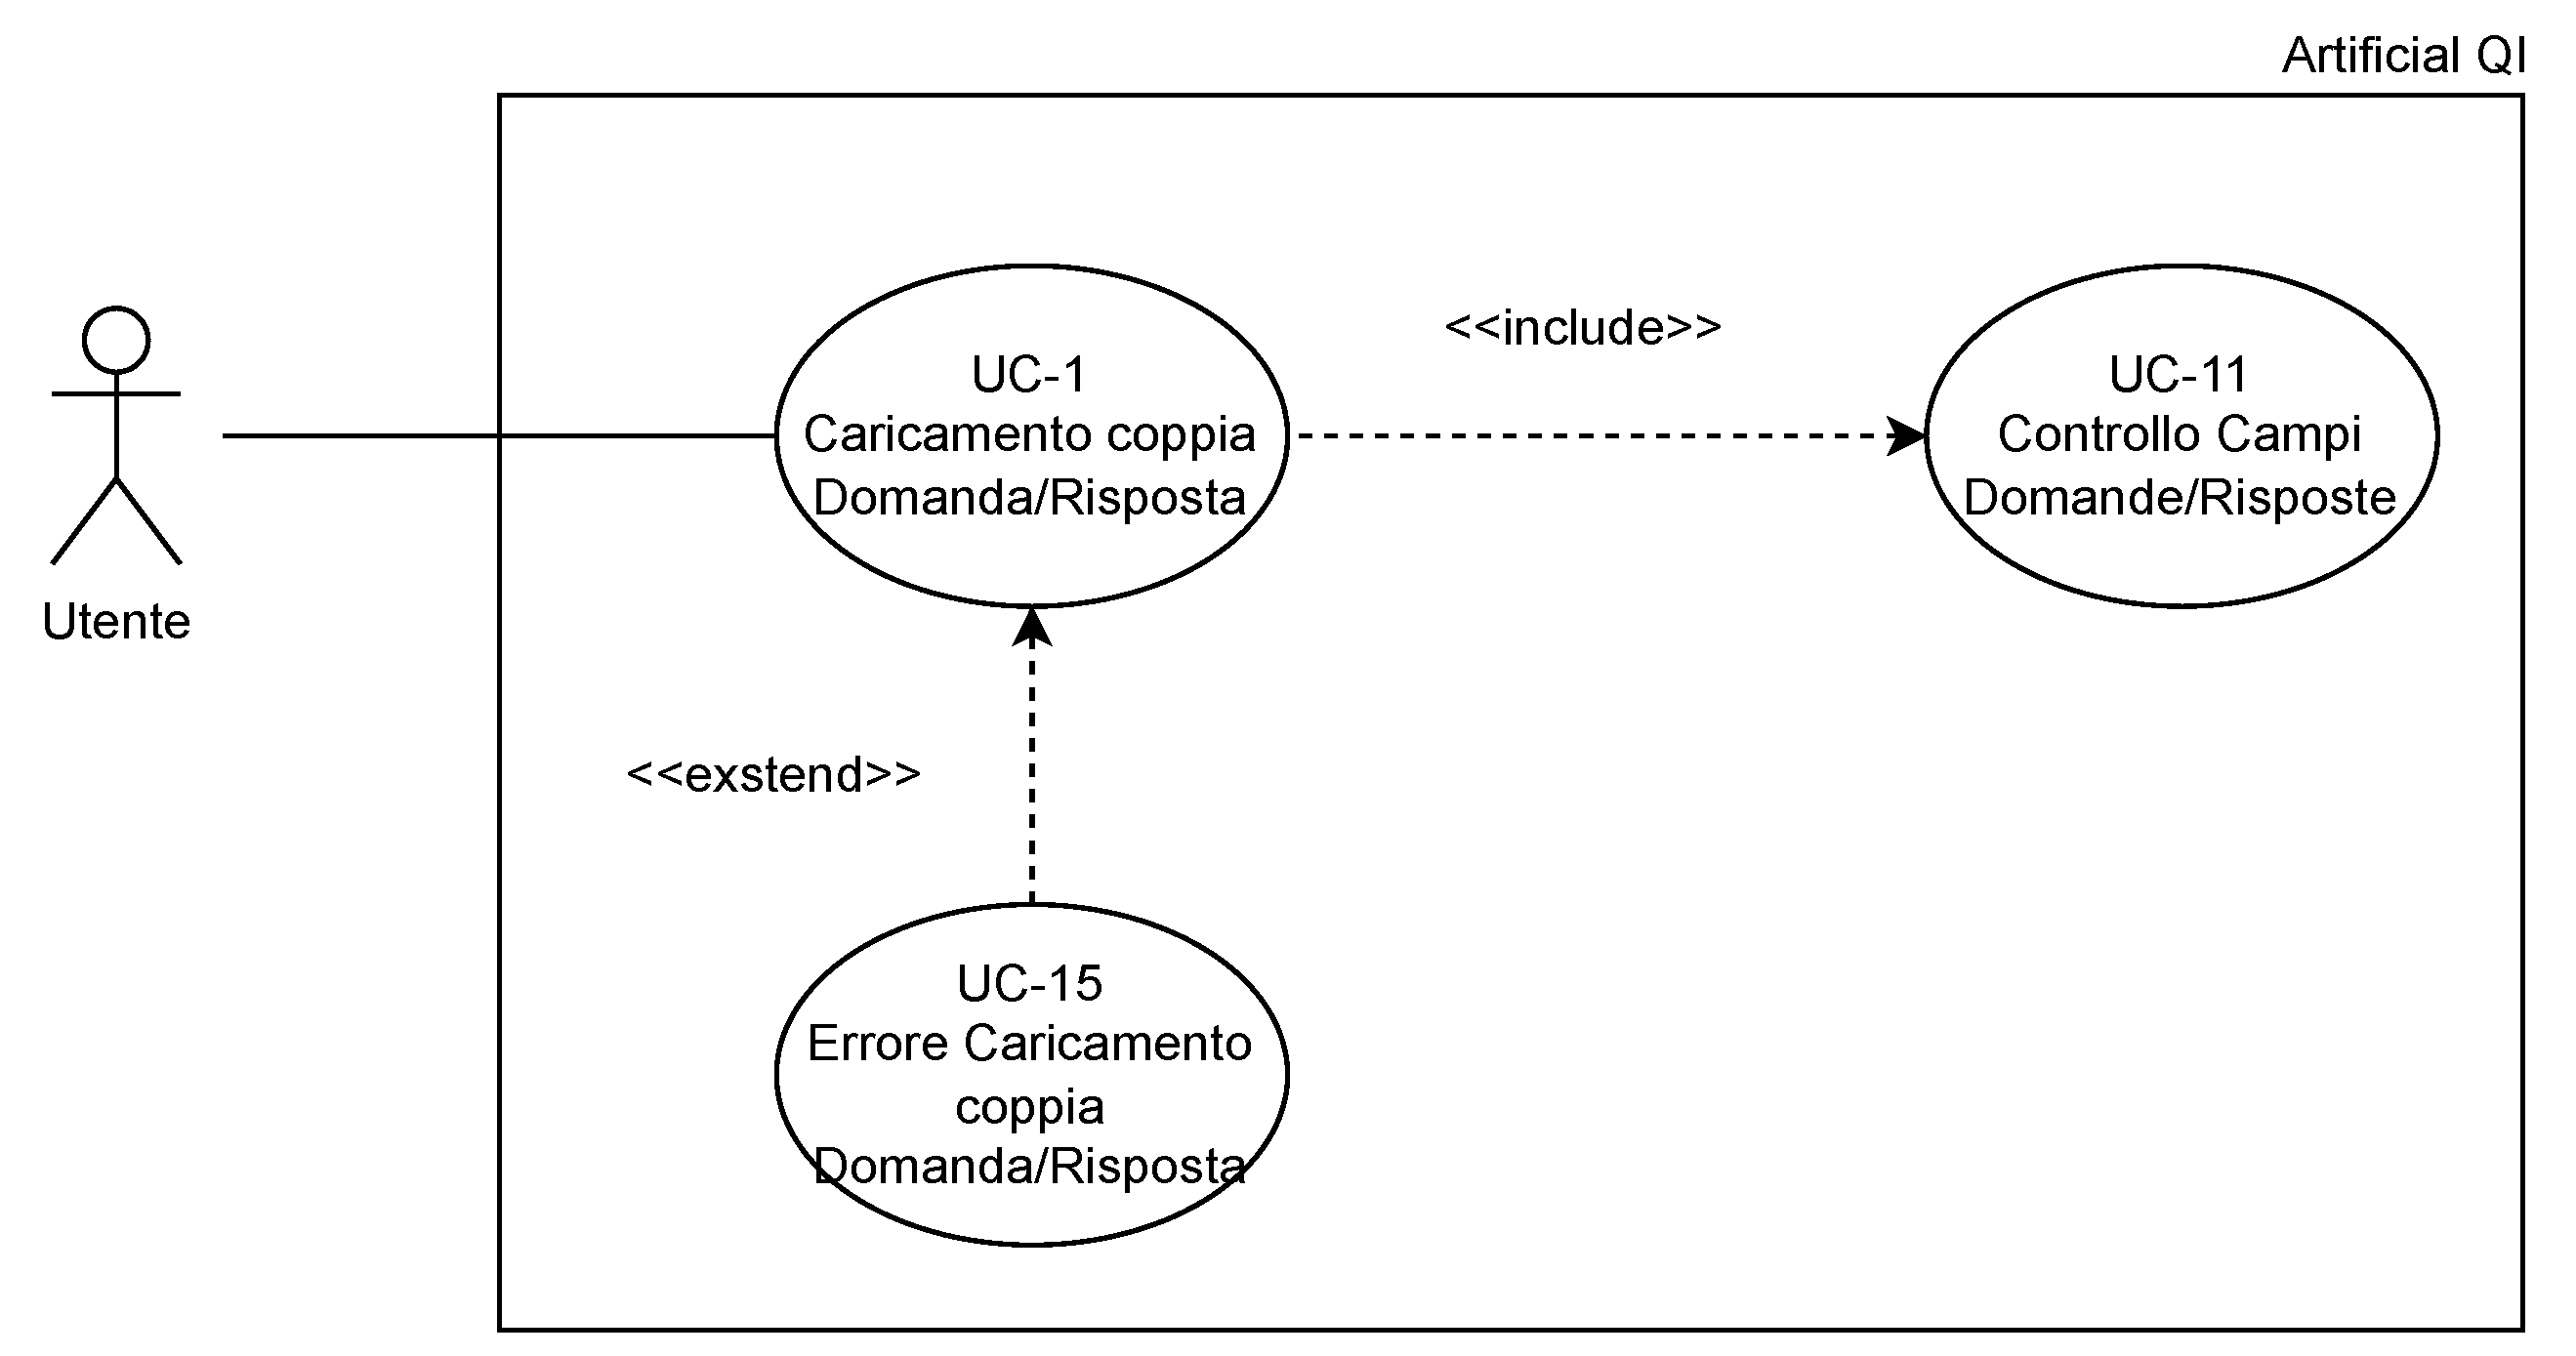
\includegraphics[width=0.8\textwidth]{../Immagini/UC-1.png}
    \caption{Diagramma dei Casi d'Uso per UC-1: Inserimento di coppie domanda-risposta}
    \label{fig:uc1-diagram}
\end{figure}

\subsubsection{UC-2: Modifica di coppie domanda-risposta}
\begin{itemize}
    \item \textbf{Precondizioni:} Esistono coppie nel sistema.
    \item \textbf{Postcondizioni:} La domanda o risposta è stata modificata e salvata.
    \item \textbf{Attori principali:} Operatore.
    \item \textbf{Attori secondari:} Sistema.
    \item \textbf{Trigger:} L'operatore seleziona una coppia da modificare.
    \item \textbf{User Story:} Come operatore, voglio modificare una domanda o risposta per correggere errori o aggiornare i contenuti.
    \item \textbf{Scenario principale:}
    \begin{enumerate}
        \item L'operatore visualizza l'elenco delle coppie.
        \item Seleziona una coppia da modificare.
        \item Apporta le modifiche.
        \item Conferma l'operazione.
        \item Il sistema salva le modifiche e notifica il successo.
    \end{enumerate}
    \item \textbf{Scenario alternativo:}
    \begin{enumerate}
        \item[4a.] L'operatore abbandona l'operazione.
        \item[4a1.] Il sistema annulla le modifiche.
    \end{enumerate}
\end{itemize}
\begin{figure}[hbt!]
    \centering
    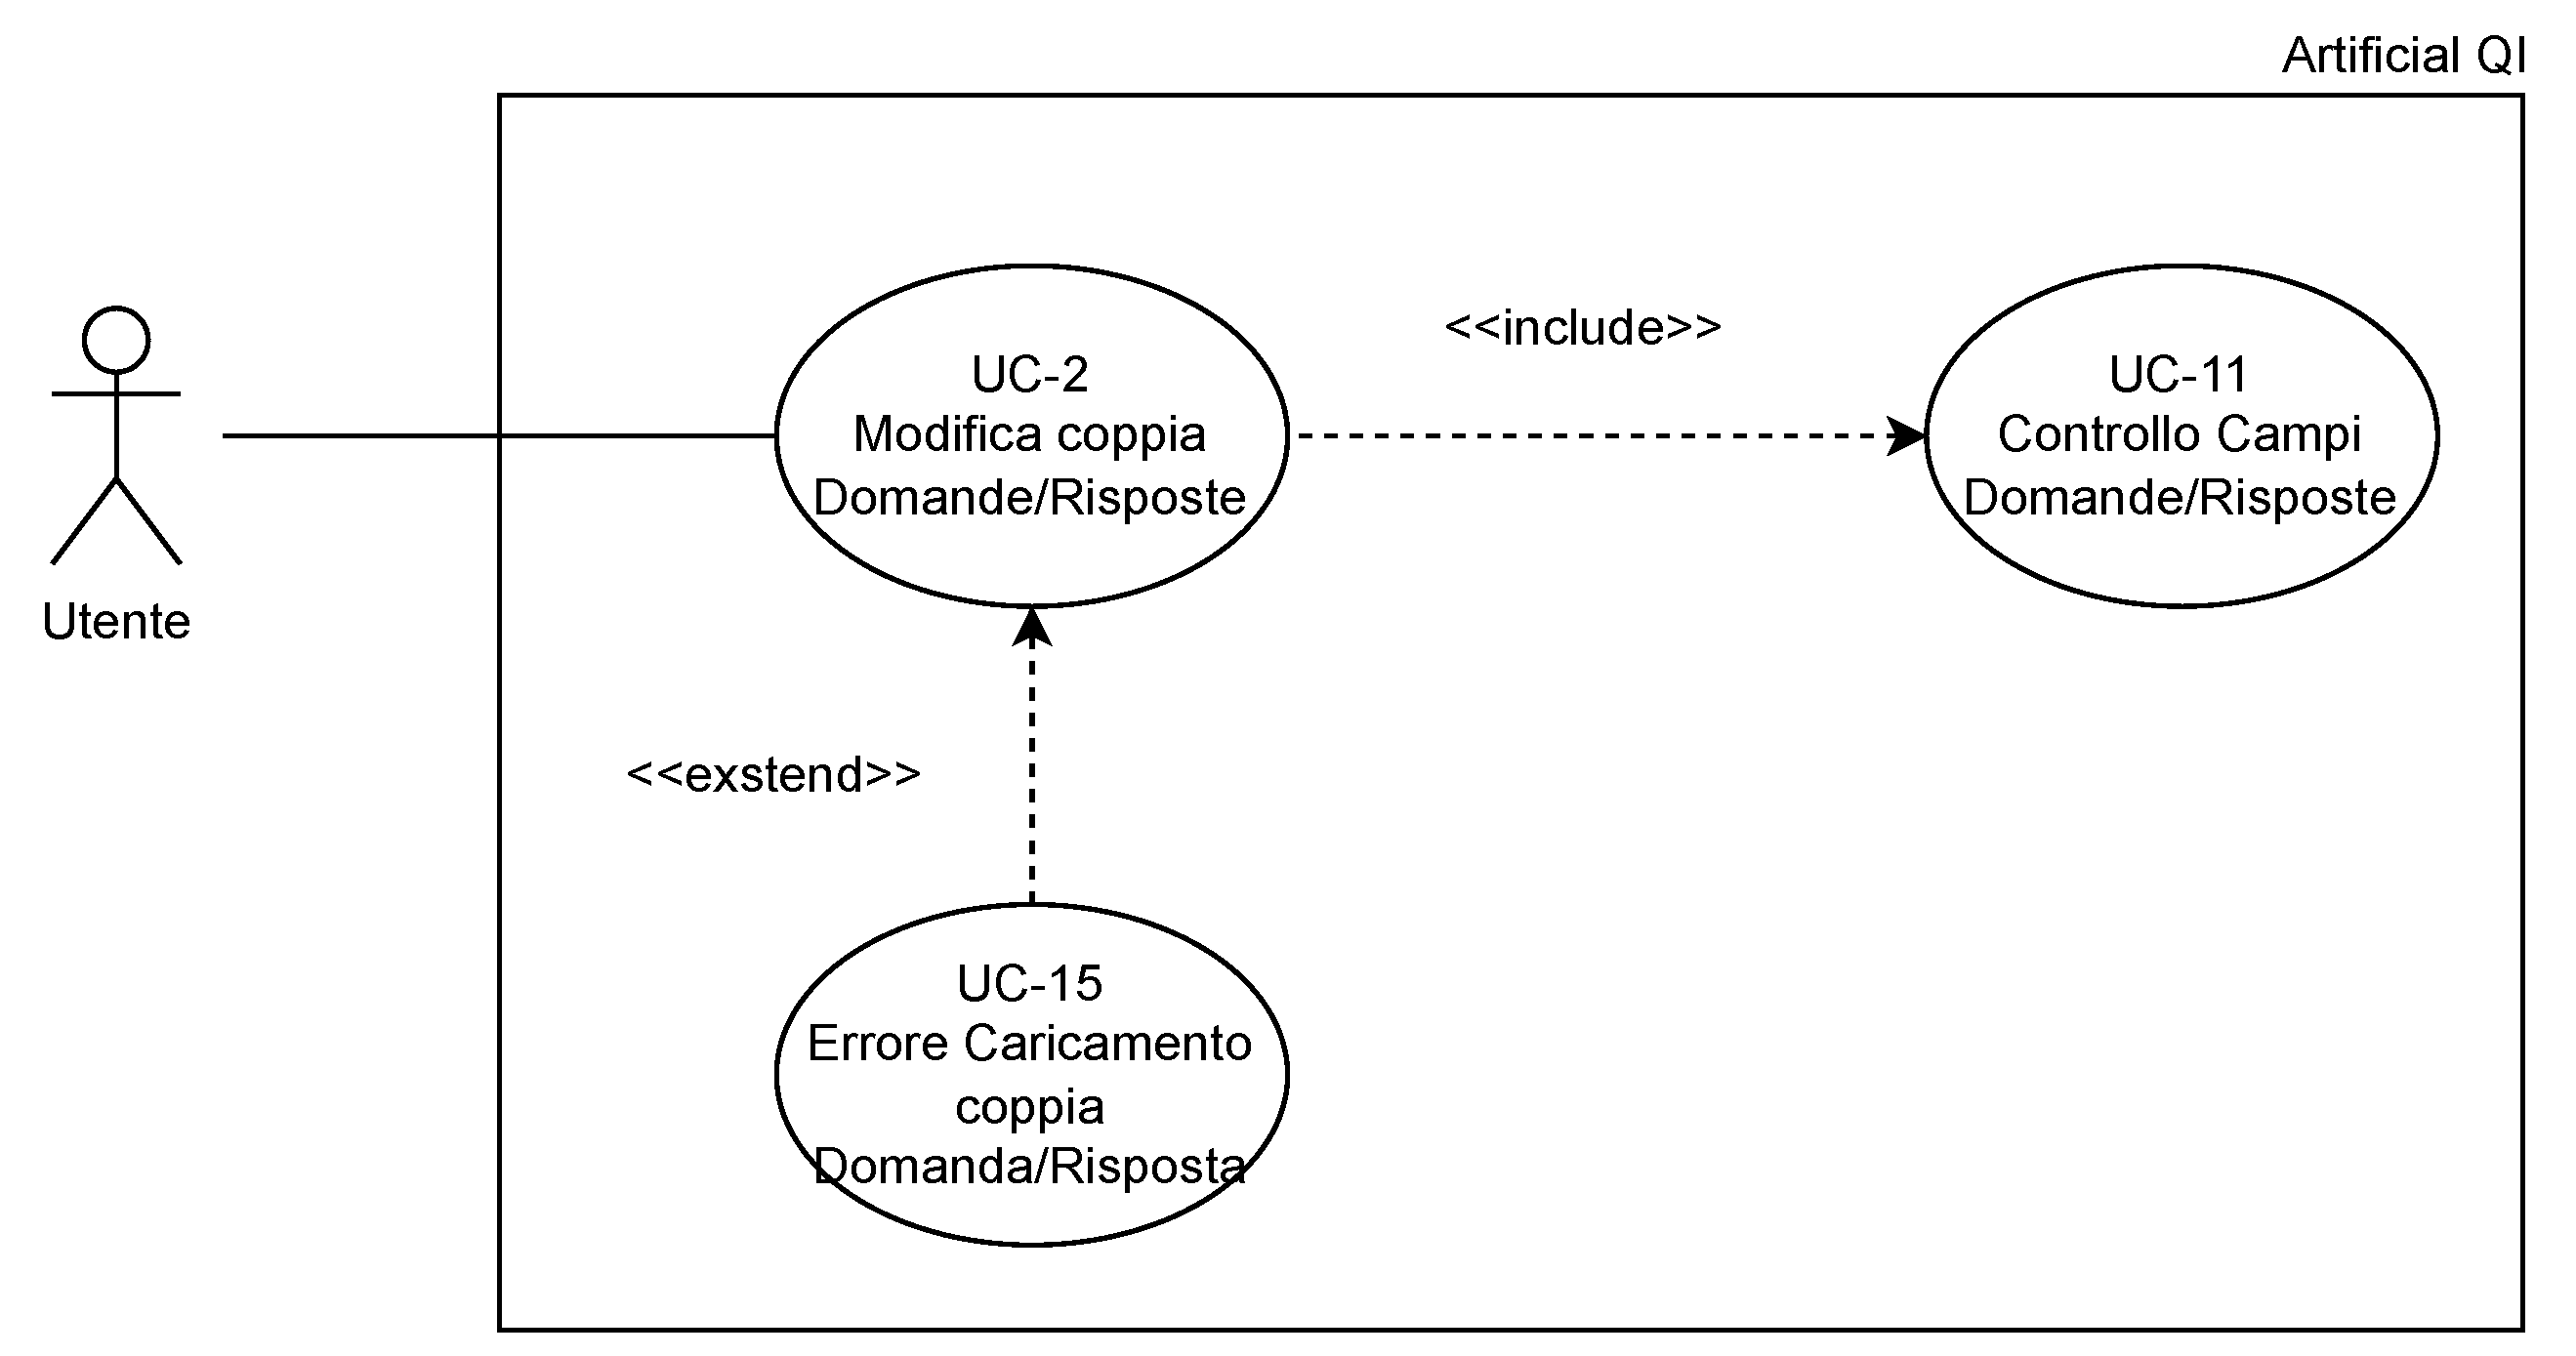
\includegraphics[width=0.8\textwidth]{../Immagini/UC-2.png}
    \caption{Diagramma dei Casi d'Uso per UC-2: Modifica di coppie domanda-risposta}
    \label{fig:uc1-diagram}
\end{figure}

\subsubsection{UC-3: Eliminazione di coppie domanda-risposta}
\begin{itemize}
    \item \textbf{Precondizioni:} Esistono coppie nel sistema.
    \item \textbf{Postcondizioni:} La coppia selezionata è stata rimossa.
    \item \textbf{Attori principali:} Operatore.
    \item \textbf{Attori secondari:} Sistema.
    \item \textbf{Trigger:} L'operatore seleziona una coppia da eliminare.
    \item \textbf{User Story:} Come operatore, voglio eliminare una coppia domanda-risposta per rimuovere contenuti obsoleti.
    \item \textbf{Scenario principale:}
    \begin{enumerate}
        \item L'operatore visualizza l'elenco delle coppie.
        \item Seleziona una coppia da eliminare.
        \item Conferma l'eliminazione.
        \item Il sistema rimuove la coppia e notifica il successo.
    \end{enumerate}
    \item \textbf{Scenario alternativo:}
    \begin{enumerate}
        \item[3a.] L'operatore non conferma l'eliminazione.
        \item[3a1.] Il sistema annulla l'operazione.
    \end{enumerate}
\end{itemize}

\subsubsection{UC-4: Ricerca di coppie domanda-risposta}
\begin{itemize}
    \item \textbf{Precondizioni:} Esistono coppie domanda-risposta nel sistema.
    \item \textbf{Postcondizioni:} L'elenco delle coppie che corrispondono ai criteri di ricerca viene visualizzato.
    \item \textbf{Attori principali:} Operatore.
    \item \textbf{Attori secondari:} Sistema.
    \item \textbf{Trigger:} L'operatore avvia una ricerca inserendo criteri specifici.
    \item \textbf{User Story:} Come operatore, voglio cercare una coppia domanda-risposta per localizzare rapidamente informazioni specifiche.
    \item \textbf{Scenario principale:}
    \begin{enumerate}
        \item L'operatore accede alla funzione di ricerca.
        \item Inserisce i criteri di ricerca (domanda, risposta o entrambi).
        \item Conferma la ricerca.
        \item Il sistema restituisce l'elenco delle coppie corrispondenti.
    \end{enumerate}
    \item \textbf{Scenario alternativo:}
    \begin{enumerate}
        \item[3a.] Non esistono coppie corrispondenti ai criteri.
        \item[3a1.] Il sistema notifica che non sono stati trovati risultati.
    \end{enumerate}
\end{itemize}

\subsubsection{UC-5: Archiviazione di un insieme di coppie domanda-risposta}
\begin{itemize}
    \item \textbf{Precondizioni:} Esistono coppie domanda-risposta nel sistema.
    \item \textbf{Postcondizioni:} L'insieme selezionato è stato archiviato.
    \item \textbf{Attori principali:} Operatore.
    \item \textbf{Attori secondari:} Sistema.
    \item \textbf{Trigger:} L'operatore seleziona un insieme di coppie per archiviarle.
    \item \textbf{User Story:} Come operatore, voglio archiviare un insieme di coppie domanda-risposta per organizzarle meglio.
    \item \textbf{Scenario principale:}
    \begin{enumerate}
        \item L'operatore seleziona le coppie da archiviare.
        \item Conferma l'archiviazione.
        \item Il sistema sposta le coppie nell'archivio designato.
    \end{enumerate}
    \item \textbf{Scenario alternativo:}
    \begin{enumerate}
        \item[2a.] L'operatore annulla l'operazione.
        \item[2a1.] Il sistema non apporta alcuna modifica.
    \end{enumerate}
\end{itemize}

\subsubsection{UC-6: Visualizzazione di un insieme di coppie domanda-risposta}
\begin{itemize}
    \item \textbf{Precondizioni:} Esistono coppie domanda-risposta nel sistema.
    \item \textbf{Postcondizioni:} L'insieme selezionato di coppie domanda-risposta viene visualizzato all'operatore.
    \item \textbf{Attori principali:} Operatore.
    \item \textbf{Attori secondari:} Sistema.
    \item \textbf{Trigger:} L'operatore seleziona l'opzione per visualizzare un insieme di coppie domanda-risposta.
    \item \textbf{User Story:} Come operatore, voglio visualizzare un insieme di coppie domanda-risposta per consultare i contenuti e analizzare le risposte archiviate.
    \item \textbf{Scenario principale:}
    \begin{enumerate}
        \item L'operatore accede alla funzione di visualizzazione.
        \item Seleziona un insieme di coppie domanda-risposta da consultare.
        \item Il sistema recupera e mostra l'elenco delle coppie selezionate.
    \end{enumerate}
    \item \textbf{Scenario alternativo:}
    \begin{enumerate}
        \item[2a.] L'operatore non seleziona alcun insieme.
        \item[2a1.] Il sistema richiede di selezionare un insieme per poter procedere.
    \end{enumerate}
\end{itemize}

\subsubsection{UC-7: Modifica di un insieme di coppie domanda-risposta archiviate}
\begin{itemize}
    \item \textbf{Precondizioni:} Esistono coppie archiviate nel sistema.
    \item \textbf{Postcondizioni:} Le modifiche apportate alle coppie selezionate sono state salvate.
    \item \textbf{Attori principali:} Operatore.
    \item \textbf{Attori secondari:} Sistema.
    \item \textbf{Trigger:} L'operatore seleziona un insieme di coppie archiviate per modificarle.
    \item \textbf{User Story:} Come operatore, voglio modificare un insieme di coppie archiviate per aggiornare i dati.
    \item \textbf{Scenario principale:}
    \begin{enumerate}
        \item L'operatore accede all'archivio.
        \item Seleziona l'insieme di coppie da modificare.
        \item Apporta le modifiche necessarie.
        \item Conferma l'operazione.
        \item Il sistema salva le modifiche.
    \end{enumerate}
    \item \textbf{Scenario alternativo:}
    \begin{enumerate}
        \item[3a.] L'operatore annulla l'operazione.
        \item[3a1.] Il sistema non salva le modifiche.
    \end{enumerate}
\end{itemize}

\subsubsection{UC-8: Eliminazione di un insieme di coppie domanda-risposta archiviate}
\begin{itemize}
    \item \textbf{Precondizioni:} Esistono coppie archiviate nel sistema.
    \item \textbf{Postcondizioni:} Le coppie selezionate sono state rimosse dall'archivio.
    \item \textbf{Attori principali:} Operatore.
    \item \textbf{Attori secondari:} Sistema.
    \item \textbf{Trigger:} L'operatore seleziona un insieme di coppie archiviate per eliminarle.
    \item \textbf{User Story:} Come operatore, voglio eliminare un insieme di coppie archiviate per mantenere l'archivio aggiornato e ordinato.
    \item \textbf{Scenario principale:}
    \begin{enumerate}
        \item L'operatore accede all'archivio.
        \item Seleziona le coppie da eliminare.
        \item Conferma l'eliminazione.
        \item Il sistema rimuove le coppie selezionate.
    \end{enumerate}
    \item \textbf{Scenario alternativo:}
    \begin{enumerate}
        \item[3a.] L'operatore annulla l'operazione.
        \item[3a1.] Il sistema non elimina le coppie.
    \end{enumerate}
\end{itemize}

\subsubsection{UC-9: Esecuzione del test su un insieme di coppie domanda-risposta}
\begin{itemize}
    \item \textbf{Precondizioni:} Esistono coppie domanda-risposta nel sistema.
    \item \textbf{Postcondizioni:} Il test è stato eseguito e i risultati sono stati generati.
    \item \textbf{Attori principali:} Operatore.
    \item \textbf{Attori secondari:} Sistema.
    \item \textbf{Trigger:} L'operatore avvia un test.
    \item \textbf{User Story:} Come operatore, voglio eseguire un test sulle coppie domanda-risposta per verificare l'efficacia delle risposte.
    \item \textbf{Scenario principale:}
    \begin{enumerate}
        \item L'operatore seleziona le coppie su cui eseguire il test.
        \item Avvia il test.
        \item Il sistema esegue il test e restituisce i risultati.
    \end{enumerate}
    \item \textbf{Scenario alternativo:}
    \begin{enumerate}
        \item[2a.] Il sistema rileva un errore nell'esecuzione del test.
        \item[2a1.] Il sistema notifica l'errore e fornisce dettagli.
    \end{enumerate}
\end{itemize}

\subsubsection{UC-10: Visualizzazione dei risultati del test}
\begin{itemize}
    \item \textbf{Precondizioni:} Esistono risultati di test disponibili nel sistema.
    \item \textbf{Postcondizioni:} L'operatore visualizza i risultati del test selezionato.
    \item \textbf{Attori principali:} Operatore.
    \item \textbf{Attori secondari:} Sistema.
    \item \textbf{Trigger:} L'operatore seleziona i risultati di un test per visualizzarli.
    \item \textbf{User Story:} Come operatore, voglio visualizzare i risultati del test per valutare le performance delle risposte.
    \item \textbf{Scenario principale:}
    \begin{enumerate}
        \item L'operatore accede alla sezione risultati.
        \item Seleziona il test di interesse.
        \item Visualizza i risultati dettagliati.
    \end{enumerate}
\end{itemize}
\begin{figure}[hbt!]
    \centering
    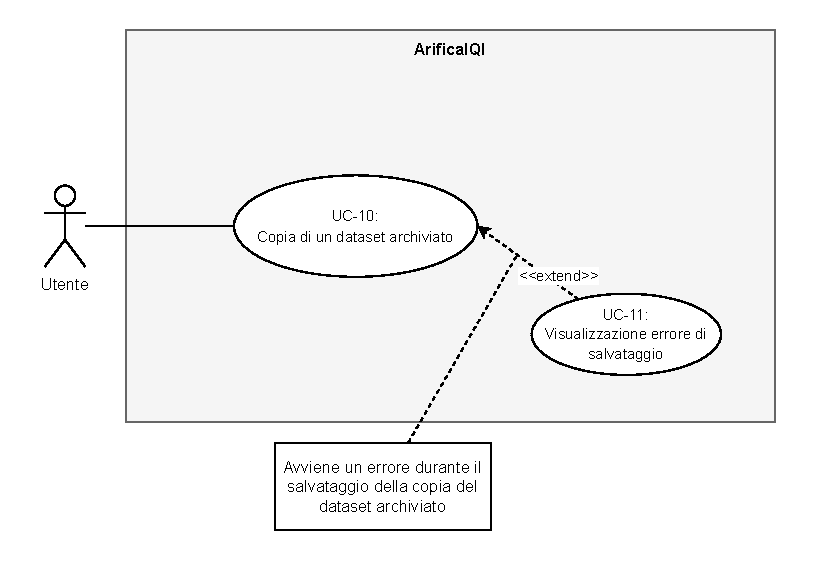
\includegraphics[width=0.8\textwidth]{../Immagini/UC-10.png}
    \caption{Diagramma dei Casi d'Uso per UC-10: Visualizzazione dei risultati del test}
    \label{fig:uc1-diagram}
\end{figure}

\end{document}